\documentclass[a4paper,12pt]{article}

% Packages
\usepackage[utf8]{inputenc}
\usepackage[T1]{fontenc}
\usepackage{amsmath}
\usepackage{amssymb}
\usepackage{graphicx}
\usepackage{hyperref}
\usepackage{parskip}
\usepackage{animate}
\usepackage{comment}
\usepackage{subcaption}
\usepackage{geometry}
\geometry{margin=1in}

% Title and Author
\title{Flow Matching}
\author{Samy Braik}
\date{\today}

\begin{document}

\maketitle

\section{Notations}
We start by defining a probability density path \(p:[0,1]\times\mathbb{R}^d\rightarrow\mathbb{R}^d\) meaning that for each time \(t\), \(p_t\) is density function i.e. \(\int p_t(x)dx=1\).\\
A simple example of such a path is a path \(p\) interpolating two density \(p_0\) and \(p_1\) with \(p_t=tp_1+(1-t)p_0\)

\begin{comment}
\begin{figure}[h]
    \centering
    \animategraphics[autoplay,loop,width=1\linewidth]{10}{frame_}{000}{019}
    \caption{Probability path interpolating $\mathcal{N}(0,0.2)$ and $\mathcal{U}([0,1])$}
    \label{fig:interpolated_density}
\end{figure}
\end{comment}

\begin{figure}[htbp]
    \centering
    \begin{subfigure}[b]{0.45\textwidth}
      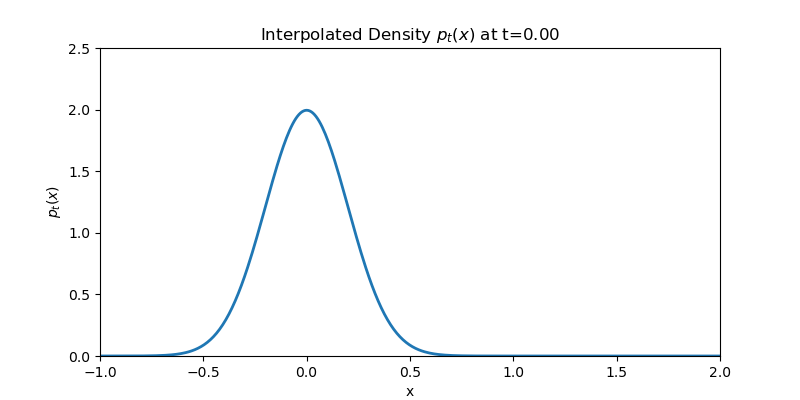
\includegraphics[width=\linewidth]{frames/frame_1.png}
      \caption{}
    \end{subfigure}
    \hfill
    \begin{subfigure}[b]{0.45\textwidth}
      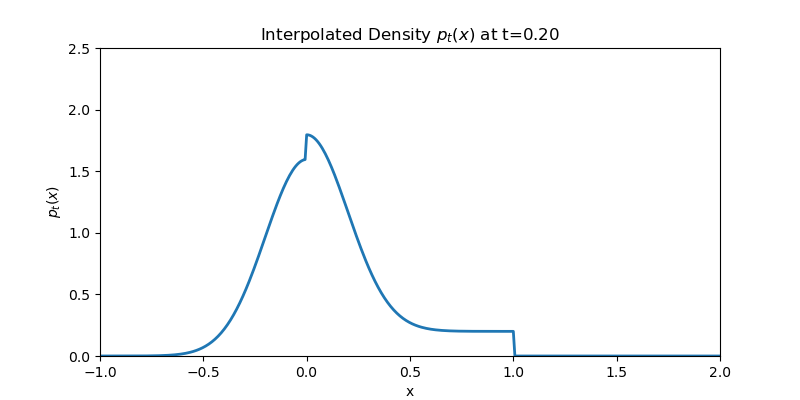
\includegraphics[width=\linewidth]{frames/frame_2.png}
      \caption{}
    \end{subfigure}
    \par\medskip
    \begin{subfigure}[b]{0.45\textwidth}
      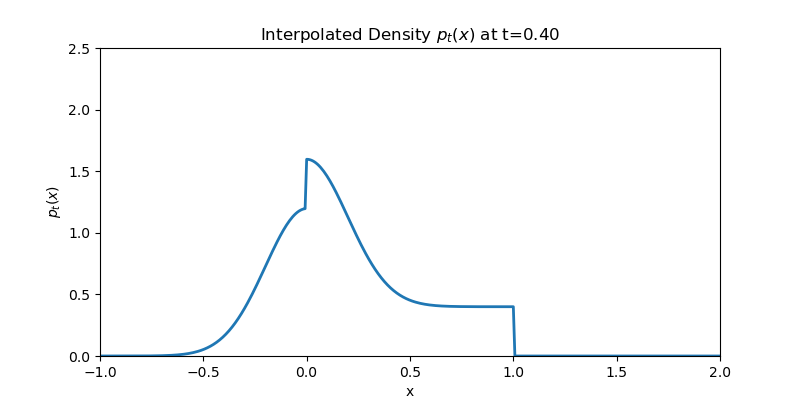
\includegraphics[width=\linewidth]{frames/frame_3.png}
      \caption{}
    \end{subfigure}
    \hfill
    \begin{subfigure}[b]{0.45\textwidth}
      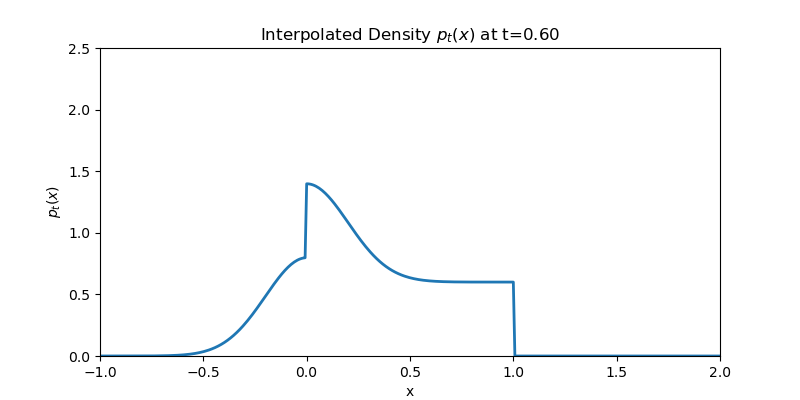
\includegraphics[width=\linewidth]{frames/frame_4.png}
      \caption{}
    \end{subfigure}
    \par\medskip
    \begin{subfigure}[b]{0.45\textwidth}
      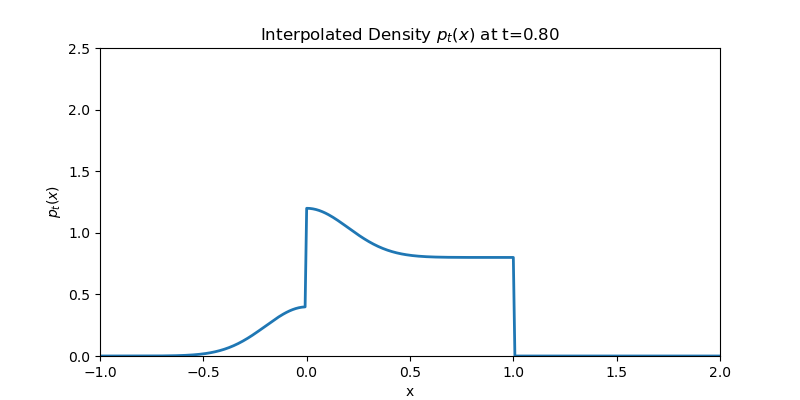
\includegraphics[width=\linewidth]{frames/frame_5.png}
      \caption{}
    \end{subfigure}
    \hfill
    \begin{subfigure}[b]{0.45\textwidth}
      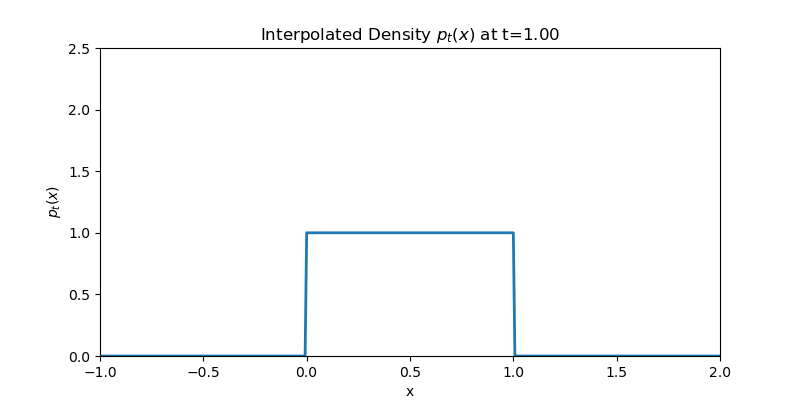
\includegraphics[width=\linewidth]{frames/frame_6.png}
      \caption{}
    \end{subfigure}
    \caption{A probability path interpolating $\mathcal{N}(0,0.2)$ and $\mathcal{U}([0,1])$}
    \label{fig:interpolated_density}
\end{figure}

\newpage

Next we introduce a core object, a time dependant vector field \(v:[0,1]\times \mathbb{R}^d\rightarrow\mathbb{R}^d\) which can be used to construct a map \(\phi:[0,1]\times\mathbb{R}^d\rightarrow\mathbb{R}^d\), called a flow, by the following ODE
\begin{align}
    \frac{d}{dt}\phi_t(x)&=v_t(\phi_t(x))\\
    \quad \phi_0(x)&=x \nonumber
\end{align}  
The link between the flow and the probability path is given by the change of variables formula 
\begin{align}
    p_t(x)=q(\phi_t^{-1}(x))\det \left[\frac{\partial\phi_t^{-1}}{\partial x}(x)\right]
\end{align}
This coincides with the normalizing framework. \\
The link between the vector field and the probability path is given by the continuity equation 
\begin{align}
  \frac{d}{dt}p_t(x)+\text{div}(p_t(x)v_t(x))=0
\end{align}
It said that the vector field \(v_t\) generates the probability path \(p_t\) if the continuity equation holds.\\
\bigskip

\section{Objective}
Given a target probability path \(p_t\) and a corresponding \(v_t\) vector field, the naïve flow matching loss is 

\begin{align}
    \mathcal{L}_\text{FM}(\theta) = \mathbb{E}_{t,p_t(x)}\left[\|v_t^\theta(x)-v_t(x)\|^2\right]
\end{align}

But we don't have acces to \(v_t\) and \(p_t\). To adress this problem and given a particular data sample \(x_1\), we introduce conditional probability path \(p_t(x|x_1)\) such that \(p_0(x|x_1)=q(x)\) at time \(t=0\) and by marginalizing over \(x_1\) we can recover the marginal probability path  
\begin{align}
  p_t(x)=\int p_t(x|x_1)q(x_1)dx_1
\end{align}
in the same vein, we can define a conditional vector field, assuming \(p_t(x)\) for all \(t\) and \(x\) 
\begin{align}
  v_t(x)=\int v_t(x|x_1)\frac{p_t(x|x_1)q(x_1)}{p_t(x)}dx_1
\end{align}

Then the author introduces a new loss function called the conditional flow matching loss
\begin{align}
  \mathcal{L}_\text{CFM}(\theta) = \mathbb{E}_{t,q(x_1),p_t(x|x_1)}\left[\|v_t^\theta(x|x_1)-v_t(x|x_1)\|^2\right]
\end{align}
with a strong property : \(\mathcal{L}_\text{FM}(\theta)=\mathcal{L}_\text{CFM}(\theta)\) up to a constant independent of \(\theta\). \\
So the focus is now on designing a conditional probability path and vector field and it turns out "the conditional flow matching objective works with any choice of conditional probability path and conditional vector fields". Futhermore, there is an infinite number of vector fields that generate any particular probability path.\\

\section{Example}


\bibliographystyle{plain}
\bibliography{references}

\end{document}